\chapter{Development Process \& Contributing to MATSim}
\label{ch:developmentprocess}
% ##################################################################################################################

\hfill \textbf{Authors:} Andreas Horni, Kai Nagel, Marcel Rieser

\begin{center} 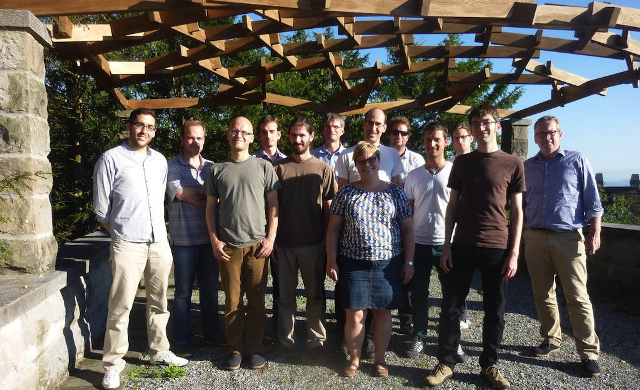
\includegraphics[width=0.5\textwidth, angle=0]{extending/figures/ConceptualMeetingVillaHatt.png} \end{center}

% ##################################################################################################################
This chapter describes how new functionality enters \gls{matsim}. It describes the \gls{matsim} team and community, the different roles existing in the \gls{matsim} project, development drivers and processes, and tools used for integration. The goal is to 
%give you 
provide an overview of the development process such that 
%you 
one quickly finds access to the \gls{matsim} community and such that 
%you are 
one is able to efficiently contribute to \gls{matsim} according to one role or another, if you commendably like to.

% ##################################################################################################################
\section{MATSim Team and MATSim Community}
The \gls{matsim} core team, 
%the heart of the \gls{matsim} community, 
currently consists of three research groups and a spin-off company, namely 
\begin{compactitem}
\item the Transport Systems Planning and Transport Telematics group at the Institute for Land and Sea Transport Systems (VSP), Technische Universität Berlin, led by Prof.~Dr.~Kai Nagel,
\item the Transport Planning group at the Institute for Transport Planning and Systems (IVT), Swiss Federal Institute of Technology Zürich, led by Prof.~Dr.~Kay~W.~Axhausen, 
\item the recently founded Mobility and Transportation Planning group at the Future Cities Laboratory, based in Singapore and led by Prof.~Dr.~Kay~W.~Axhausen, and 
\item \gls{senozon}, based at Zürich with a subsidiary in Germany, founded by former PhD and research students. 
\end{compactitem}

As common in research the universities groups' composition changes frequently. Over the last decade more than 50\,people build the \gls{matsim} core as listed earlier.

Besides the \gls{matsim} core team, there is a community composed of closely connected research groups (such as Stockholm, Pretoria, Poznan, and Jülich),
% and Toronto) 
%\kai{habe Toronto hier rausgenommen.  Spricht etwas dagegen?}
%\ah{nein. Danke! }
and more loosely connected external users coming together, e.g., at the annual \gls{matsim} user meeting.   

\gls{matsim} is an open-source program provided by the \gls{gplv2}, thus, you are also very welcome to contribute to the code base as described in Section~\ref{sec:yourcontribution}. New contributors are mentored in the beginning \citep[][]{MATSIM-BecomingAContributor_Webpage_2015} to become familiar with the project and the coding conventions \citep[][]{MATSIM-CodingGuide_Webpage_2015}.

Picture~\ref{fig:team} shows a snapshot of the participants of the first conceptual meeting representing a good mix of core group members but also associated researchers.
%
% ------------
\createfigure%
{Participants of the first MATSim conceptual meeting at Villa Hatt in Zürich in 2012}%
{Participants of the first MATSim conceptual meeting at Villa Hatt in Zürich in 2012}%
{\label{fig:team}}%
{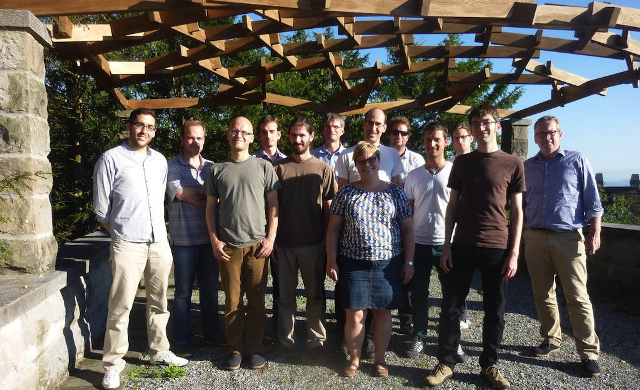
\includegraphics[width=0.99\textwidth, angle=0]{extending/figures/ConceptualMeetingVillaHatt.png}}%
{}
% ------------

% ##################################################################################################################
\section{Roles in the MATSim community}
\label{sec:roles}
There are the following roles in the \gls{matsim} community.
%
\begin{compactitem}
\item The \textbf{\gls{matsim} user} uses the official releases or nightly builds and runs \gls{matsim} with the config file. Part~I of the book is dedicated to the \gls{matsim} user. On the web page he or she finds relevant information in the \emph{user's guide} and in the user's mailing list \lstinline|matsim-users@lists.sourceforge.net|.
%
Part~III of the book discusses conceptual issues, including Chapter~\ref{ch:researchavenues} that sketches some issues that need further development.
%
\item The \textbf{\gls{matsim} \gls{api}-user} extends \gls{matsim} by programming against the \gls{matsim}-\gls{api}. He or she finds his or her information in Part~II of the book, in particular in Chapter~\ref{ch:extensionpoints}, on the web page in the \emph{\gls{api}-user's guide} and in the mailing list \lstinline|matsim-devel@lists.sourceforge.net|.
%
\item The \textbf{\gls{matsim} API-developer} also programs against the \gls{matsim}-\gls{api}, but additionally he or she is part of the \gls{matsim} code base by having his or her own playground or \gls{contribution} being part of the refactorings. 
%\ah{contribs auch, oder?} \kai{ja}. 
The API-developer finds information in Part~II of this book, on the web page in the \emph{developer's guide} and in the mailing list \lstinline|matsim-devel@lists.sourceforge.net| 
%
\item There are relatively few \textbf{\gls{matsim} core developers} stemming from the \gls{matsim} team. This role is an extension of the \gls{matsim} API-developer and these guys make necessary modifications of the core code (\lstinline|package org.matsim.core.*| see next section), usually after having discussed them in the issue tracker, in the \gls{matsim} committee, or at a developer meeting (see below). 
%% Part~II and part~III of this book might be particularly interesting for them.
%
% \kn{Sehe nicht, warum ausgerechnet die core developers neben dem software engineering auch noch die mathematisch-konzeptionelle Arbeit übernehmen müssen. --> weglassen}
% \ah{Dachte eher an Hintergrund: Damit man auch weiss, was man in einem weiteren Sinn eigentlich tut. Gibt aber verschiedene Blickwinkel drauf ... und deinen finde ich mittlerweile viel naheliegender.}

\end{compactitem}
%
% ##################################################################################################################
\section{Drivers and Organization of Development}
Main drivers of the \gls{matsim} development are the projects and dissertations accomplished by the \gls{matsim} team. New features are developed as an answer to requirements of these dissertations and projects, where projects range 
%
from purely scientific ones (often sponsored by \gls{snf} or \gls{dfg}) 
%
via projects for governmental entities
%administration 
%
and projects where science and industry contribute equally (e.g.\ \gls{cti}-projects) 
%
to purely 
%industrial 
commercial projects, which are managed by \gls{senozon} in the majority of cases. 
%
A significant amount of innovation is also introduced by the collaboration with external researchers.

Systematic code integration is mainly performed by the Berlin group and by \gls{senozon}. This includes continuous code review and integration upon request of the community, but also comprehensive code refactorings to clean up
%degenerated 
code and to 
improve modularity.  Refactorings are discussed and documented in the \gls{matsim} issue tracker.

The development process is supported by a standing \gls{matsim} committee discussing conceptual issues on a regular basis. Another element bringing in innovation but also organization are the annual meetings. Right from the beginnings, there has been a \gls{matsim} developer meeting focused on coding issues. Later, a user meeting giving insights into accomplished work by the community has been invented. Finally, a conceptual meeting has been added strictly dedicated to issues that go beyond pure software engineering. The developer and the conceptual meeting have shown to establish an effective road map, which has guided the development for the remainder of the year. 

The internal development is organized by regular group meetings, in Zürich for example by the "\gls{matsim} group meeting".
%% and in Berlin by the "jour fix". 

Due to the heterogeneous character of the community and its individual research groups, with every member being engaged in his individual dissertation work, organizing the development in an agile and somewhat ad hoc manner has been regarded beneficial over adopting an established and strict software project management method.

% ##################################################################################################################
\section{Code Base, Development Tools and Techniques}

% ====================================================================================
\subsection{Core, Contribs, and Playgrounds}

The various pieces of \gls{matsim} are delineated by \gls{maven} projects and sub-projects.  The \gls{maven} layout corresponds to the layout of the \gls{svn} repository.  Note that the \gls{java} package structure does \emph{not} directly correspond to the \gls{maven}/\gls{svn} layout.

\subsubsection{Core}

The so-called \gls{matsim} core corresponds to the "matsim" part of the \gls{svn} repository.  It is currently at \gls{sourceforge} under \url{https://svn.code.sf.net/p/matsim/source/matsim}. The exact path name sometimes changes, e.g., because of changes at \gls{sourceforge}.

Most of the core material is in packages that start with
\begin{compactitem}
\item \lstinline{org.matsim.api.*}
\item \lstinline{org.matsim.core.*}
\item \lstinline{tutorial.*}
\end{compactitem}
This is the material that the core developers consider most important. 

There is additional material in that part of the repository, for example under \lstinline{org.matsim.withinday.*} or \lstinline{org.matsim.pt.*}, that could as well be moved into the "contrib" section, but for the time being has remained in the core, mostly because the maintainers of these parts have moved to \gls{senozon} and from there continue to maintain these functionalities.

\subsubsection{Contrib}

%% Additionally, there is not directly related to the core functionality of \gls{matsim}, which is agent-behavior and transport simulation, 
More material, often denoted as "contrib", is in the "contrib" part of the \gls{svn} repository.  It is currently at \gls{sourceforge} under \url{https://svn.code.sf.net/p/matsim/source/contrib}.  The \gls{java} packages often have the root \lstinline{org.matsim.contrib.*}, but this is not enforced.


%% in the code base 
%% as \gls{matsim} contributions (\lstinline|package org.matsim.contrib.*|). Such modules are usually provided by \gls{matsim} \gls{api}-users or developers. %

\subsubsection{Playgrounds}

Finally, there is the "playgrounds" part of the repository.  These are meant as a service to developers.  The have historically grown from the fact that \gls{matsim}'s object classes and in consequence the interfaces between them have evolved and grown over time, and thus a stable \gls{api} was not available.  At this point, the extension points described in Chapter~\ref{ch:extensionpoints} should be somewhat stable, and development against them should be possible without major changes from release to release.  Anybody who needs tighter integration with the project should apply for a playground of her or his own.  

% ====================================================================================
\subsection{Releases, Nightly Builds and Code HEAD}
\label{sec:releases-builds}

Twice a year, a \gls{matsim} release is published, which can be downloaded from \gls{sourceforge} at \url{http://sourceforge.net/projects/matsim/files/}. Usually, \gls{matsim} users and \gls{matsim}-\gls{api}-users as defined above in Section~\ref{sec:roles} work with releases. 

MATSim is based on continuous integration and, thus, nightly builds are available without stability guarantee \url{http://matsim.org/downloads/nightly}. Nightly builds might be used by \gls{matsim}-\gls{api} users, which depend on a very recent feature. 

Only \gls{matsim} developers---either programming in their playground, in a \gls{contribution}, or in the core---work on the code's HEAD version, which is available from \gls{sourceforge} at \url{http://sourceforge.net/p/matsim/source/HEAD/tree/}.

Nightly builds are only generated when the code compiles and passes the regression tests.  They are, in consequence, somewhat "safer" than the direct download from the HEAD.

% ====================================================================================
\subsection{Development Tools}
%\kai{Moved some material from here to ``history''.}
%\ah{ok. Adapted title, as there was nothing about "core" here anyamore.}

\gls{matsim} development makes use of a whole bunch of tools greatly leading to better software quality. Summarized and accessible from \url{http://matsim.org/developer}:
%---with private access---
%
%m.E. war das nie non-public.  Evtl. nicht auf der home page ausgewiesen. kai, dec'14
a change log, an issue tracker, the \gls{javadoc}, static code analyses performed by \emph{FindBugs} and \emph{PMD}, test code coverage analysis, copy paste analysis, code metrics, \gls{maven} dependencies, the complete code linked by \gls{xref}, and the information about the nightly test results are provided. These nightly test results are generated by the \gls{matsim} build server based on \gls{jenkins}. 

Furthermore, there is a \gls{matsim} benchmark available \url{http://www.matsim.org/docs/devguide/optimization}.

Most \gls{matsim} developers use \gls{eclipse} as an \gls{ide}. The \gls{matsim} documentation is tailored to this \gls{ide}. Team development is based on \gls{svn}. External libraries dependencies are managed by \gls{maven}. 

% ##################################################################################################################
\section{Documentation, Dissemination and Support}
The main documentation can be found on the \gls{matsim} web page \citep[][]{MATSIM-Docu_Webpage_2015}, where information is distinctly provided in the three guides mentioned above. Additionally, a handful of tutorials is available, with the "Quickstart"-tutorial to get fast access to \gls{matsim} and the "Learning \gls{matsim} in 8\,Lessons"-tutorial, which is used for the user's meetings and hands-on tutorials in Berlin, Zürich and occasionally elsewhere, also listed on that page. 

Code documentation in form of \gls{javadoc} can be found at \citet[][]{MATSIM-Javadoc_Webpage_2015}, as \gls{xref} view \url{http://matsim.org/xref} and as doxygen documentation \url{http://matsim.org/doxygen}. %\kai{gerne auch xref und doxygen URLs: \url{http://matsim.org/xref} and \url{http://matsim.org/doxygen}.}

For fast application of \gls{matsim} some small-scale example scenarios are provided in the code base (\lstinline|folder: src/test/resources/test/scenarios/|), where recently an extended version of the well-known benchmark scenario for the City of Sioux Falls has been added \citep[][]{ChakirovFourie_TechRep_FCL_2014} (Section~\ref{ch:scenarios:siouxfalls}).

Further information is disseminated at the afore-described annual user meetings and \gls{matsim} mailing lists. Usually, also support is provided by the \gls{matsim} team via these mailing lists. Particularly active in support are the Berlin group and \gls{senozon}. A theoretical overview of all the components in \gls{matsim} is given by the numerous papers published in international journals and presented at worldwide conferences; an overview can be found at \citep[][]{MATSIM-Publications_Webpage_2015} and in this book's part~II.

Apparently, the information on \gls{matsim} is quite extensive, however, getting a complete picture as a new \gls{matsim} user requires a substantial literature search effort. Reduction of this hassle is the goal of the book at hand.

% ##################################################################################################################
\section{Your Contribution to MATSim}
\label{sec:yourcontribution}
The technical details, i.e., the \gls{matsim} extensions points, where to hook with \gls{matsim} are detailed in the next chapter. Here, the different ways of contributing to \gls{matsim} according to the roles presented in Section~\ref{sec:roles} are introduced.

As a user or \gls{api}-user, you are warmly welcome to make an important impact by reporting your achievements, needs and problems with, or bugs of, the software via the users mailing list or at the annual \gls{matsim} user meeting. 

If you would like to directly contribute to the code base of \gls{matsim} you are welcome to become a \gls{matsim} developer with your own playground or \gls{contribution}.

If you are the type of guy that likes to change the core system, you can, although it is a long way, become a \gls{matsim} core developer. Core developers are usually picked from the \gls{matsim} team. Prerequisites are a strong computer scientist background, several years of experience with \gls{matsim} and a deep understanding of large software projects.

% ##################################################################################################################
%\section{Discussion and TODOs}
%\label{sec:development_process}
%Will be commented, when chapter is finished. Make final results traceable.
%
%% --------------
%\kai{Ich würde gerne ``Development process'' und ``Contributing to MATSim'' auftrennen.  Ersteres beschreibt Dinge wie core development, regression tests, etc.  Aber ``contributing to MATSim'' sollte sich auf die extension points konzentrieren.  Vielleicht zusammen mit dem vorhergehenden Kapitel.}
%
%\kai{Bin mir allerdings beim zweiten Nachdenken nicht mehr sicher, ob das so kategorisch sein muss.  Wir sollten erstmal versuchen, ``contributing to matsim'' als logische Folge des development process zu schreiben.  Dann sind ``minimally invasive contributions'' ja gerade solche, welche die extension points verwenden.}
%
%% --------------
%\ah{Vieles noch etwas zu implizit dargestellt! -> Aufzählungen einfügen. Playgrounds! Testing! Verantwortlichkeiten!}
%
%% --------------
%\ah{Classes und Methods stabil seit Langem: 
%auf was deutet das hin? Zu wenig Innovation oder Clean-Code? Steckt zuviel in den Playgrounds, Contribs oder ist das genau richtig?
%Wurde Kernfunktionalität eingefügt und dafür weniger Zentrales (wie Evacuation) nach und nach in Contrib verschoben?}
%
%\ah{Der Drop Ende 2007, war das schon Core, API Umstruktutierung oder war das die Entfernung von G. package?}
%\kai{Entfernung von Gunnar's package.}
%
%\createfigure%
%{Code development since 2005}%
%{Code development since 2005}%
%{\label{fig:codedev}}%
%{%
  %\createsubfigure%
  %{...}%
  %{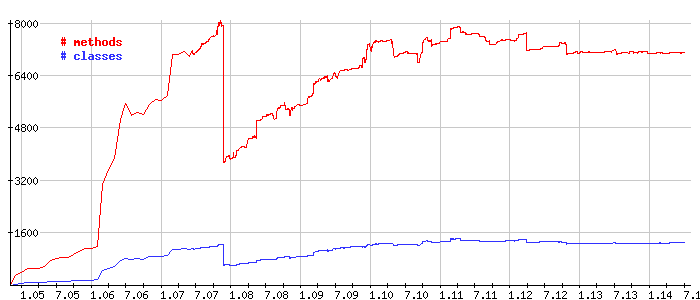
\includegraphics[width=0.95\textwidth,angle=0]{extending/figures/nof_classes.png}}%
  %{\label{fig:codedev0}}%
  %{}%
  %\createsubfigure%
  %{...}%
	%{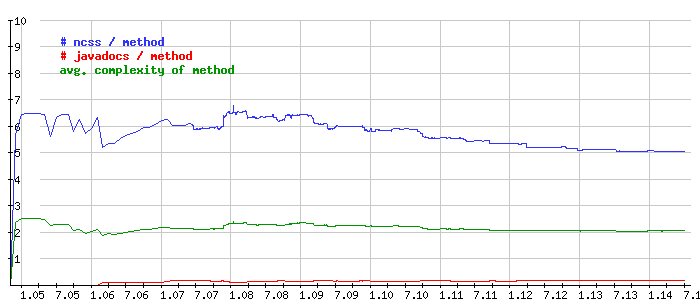
\includegraphics[width=0.95\textwidth,angle=0]{extending/figures/avg_method.png}}%
  %{\label{fig:codedev1}}%
  %{}%
%}%
%{}
%
%
%\ah{noch weiter eingehen auf Code Struktur? Resources, XML, ect.???}
%\ah{approx. number of playgrounds}
%\ah{approx number of code lines /classes at the different locations (core, playgrounds, contributions etc.}

% ##################################################################################################################
% Local Variables:
% mode: latex
% mode: reftex
% mode: visual-line
% TeX-master: "../main"
% comment-padding: 1
% fill-column: 9999
% End: 
